%-------------------- begin preamble ----------------------

\documentclass[a4paper,twocolumn]{article}

\usepackage{relsize,makeidx,color,setspace,amsmath,amsfonts,amssymb, mathtools}
\usepackage[table]{xcolor}
\usepackage{bm,ltablex,microtype}
\usepackage{hyperref}
\usepackage{fontawesome}   
\usepackage[pdftex]{graphicx}
\usepackage{tcolorbox}
\usepackage[font=small, labelfont=bf, font=footnotesize]{caption}
\usepackage{subcaption}
\usepackage{float}
\usepackage[title]{appendix}

\usepackage{setspace}

\DeclarePairedDelimiter\set\{\}
\newcommand\numberthis{\addtocounter{equation}{1}\tag{\theequation}}

% figures in multicols environment ------------------------------------------- %


\newcommand{\R}{\mathbb{R}}
\newcommand{\E}{\mathbb{E}}
\newcommand{\y}{\mathbf{y}}
\newcommand{\ytilde}{\mathbf{\widetilde{y}}}
\newcommand{\X}{\mathbf{X}}
\newcommand{\B}{\boldsymbol{\beta}}
\newcommand{\Bhat}{\boldsymbol{\hat{\beta}}}
\newcommand{\eps}{\boldsymbol{\varepsilon}}
\newcommand{\norm}[1]{\left\lVert#1\right\rVert}
\begin{titlepage}
    \begin{center}
        \Huge
        \textbf{Regression analysis and resampling methods}\\
        \vspace{0.5cm}
        \LARGE
        FYS-STK3155 - Project 1\\
        Didrik Spanne Reilstad
        
        \vspace{0.5cm}
        \begin{abstract}
            \noindent The regression methods Ordinary Least Squares, Ridge regression and Lasso regression was compared and analyzed on the Franke function with varying amounts of noise and size of datasets. While using bootstrap and k-fold cross validation as resampling techniques and MSE and the $R^{2}$-score as model assessment measurements, we found that Ordinary Least Squares performed best for larger datasets with no noise. For smaller datasets with noise, Ridge performed better and more stable for higher complexities with Lasso performing slightly worse than Ridge. After testing on the Franke function, the regression methods were applied to terrain data of an area outside Stavanger, Norway. Ordinary Least Squares estimated the terrain data best, with Ridge regression also performing well.
        \end{abstract}
        \vspace{0.8cm}
        
\includegraphics[scale=0.59]{terrain.png}
    \end{center}
\end{titlepage}

\begin{document}
\raggedbottom
\begin{center}
    \small \textbf{Github}
    
    \vspace{0.2cm}
    
    \faGithub \ \small \href{https://github.com/dreilstad/FYS-STK3155/tree/master/Project1}{github.com/dreilstad/FYS-STK3155/Project1}
\end{center}
\vspace{0.5cm}
\section{Introduction}
Regression analysis is the process of using statistical methods to examine the relationship between a number of independent variables and a dependent variable. The goal of regression analysis is to exploit the resulting model from our regression analysis to make predictions and fit a function to the independent variables. The ability to infer information from the relationship between a set of independent variables and a dependent variable to predict and forecast is an incredibly powerful tool.\\
\\
Regression analysis and modeling is widely used in disciplines such as social sciences, epidemiology, finance and economics, and also plays an important role in machine learning. Especially relevant at the time of writing, is regression analysis in the field of epidemiology. Considering the current COVID-19 pandemic, using regression analysis to track the spread of a virus in a population and being able to predict the development of spread is an incredibly powerful tool. In general regression analysis is an important tool used in analytical epidemiology.\cite{epidemiology}\\
\\
The focus of this project was to study various regression methods such as Ordinary Least Squares(OLS), Ridge regression and Lasso regression. Furthermore using resampling methods like k-fold cross validation and boostrap in order to evaluate the resulting model from the various regression methods. Code written for OLS and Ridge regression, and also for both of the aforementioned resampling methods is located in the linked Github repository. For Lasso regression, functionality from Scikit-Learn was used. \\
\\
The subsequent sections of the project starts with an outline of the theory and method used to produce the results in the present work. Also information about the datasets used in the project is provided. Thereafter the results are presented and discussed. The report is ended with a conclusion.
\section{Method}
This sections outlines the theory and method behind the regression analysis presented in the report. Including regression methods, measurements for assessing the models and resampling techniques.
\subsection{Linear regression}
Given a set of $p$ independent variables, also called characteristics or features, of $n$ samples organized in a so called design matrix $\X$. In addition where $\y$ is the observable response or outcome. If we assume a linear relationship between the independent variables of $\X$ and the response $\y$, we can fit a model using linear regression. Meaning $\y$ can be written as
\begin{equation}
    \y = \X \B + \eps
\end{equation}
The design matrix $\X$ is a matrix of size $n\times p$. The response $\y$ is a vector of size $n$ and the parameter vector $\B$ containing the linear regression coefficients $\beta_{i}$ of our model is of size $p$. The coefficients of $\B$ are unknown to us. Lastly, $\eps$ is a vector of size $n$ and represents the error term or disturbance term or sometimes noise of our model. $\eps$ contains the factors which influence the response $\y$ other than the independent variables $\mathbf{x}_{i}$, which are the columns of $\X$. $\eps$ is also assumed to be normally distributed, $\eps \sim N(0,\sigma^{2})$.\\
\\
We assume the non-trivial and more realistic situation where the $\eps$ vector contains non-zero values. . Meaning there will be a deviation between our model, denoted by $\ytilde$, and the observed values $\y$. We then write our model as
\begin{equation}
    \ytilde &= \X \B
\end{equation}
and the error or deviation between our model and the observed values $\y$ can be written as
\begin{equation}
\begin{split}
    \eps &= \y - \X \B \\
    &= \y - \ytilde
\end{split}
\end{equation}
We want to our error to be as small as possible, meaning that our model most accurately models our data. Estimating the coefficents of $\B$ such that $\eps$ is minimized, is the goal of linear regression.
\subsection{Ordinary Least Squares}
To estimate the unknown coefficients of $\B$ such that $\eps$ is minimized, we require an expression for $\B$. Using the Mean Squared Error (MSE) with the Euclidean $L^{2}$ norm for a vector space, we can write the cost function as
\begin{align*}
    C^{OLS}(\B) &= \norm{\y - \ytilde}_{2}^{2}\\
    &= \frac{1}{n}\sum_{i=0}^{n - 1} (y_{i} - \widetilde{y_{i}})^{2}\\
    &= \frac{1}{n}\set*{(\y - \ytilde)^{T}(\y - \ytilde)}\\
    &= \frac{1}{n}\set{(\y - \X\B)^{T}(\y - \X\B)}\numberthis\label{eqn}
\end{align*}
The optimal coefficients of $\B$, which we denote as $\Bhat$, is therefore
\begin{align}
    \Bhat^{OLS} = \underset{\beta}{argmin} \ C(\B)
\end{align}
In order to minimize $C(\B)$, we can differentiate the function with respect to $\B$ and set the result equal zero. We can omit the constant $\frac{1}{n}$, since it will ultimately be multiplied away. Differentiating results in
\begin{align*}
    \frac{\partial C^{OLS}(\B)}{\partial \B} &= \frac{\partial}{\partial \B}\left((\y - \X\B)^{T}(\y - \X\B)\right)\\
    &= \X^{T}(\y - \X\B) = 0
\end{align*}
and rewriting the equation yields the ordinary least squares estimator
\begin{align*}
    \X^{T}\y &= \X^{T}\X\B\\
    \Bhat^{OLS} &= \left(\X^{T}\X\right)^{-1}\X^{T}\y \numberthis\label{eqn}
\end{align*}
Equation (6), if the product $\X^{T}\X$ is invertible, provides the optimal coefficients. In section 2.1, the design matrix was defined as $\X \in \R^{n\times p}$ where $n$ samples can become quite large in our dataset because it is usually the case that $n \gg p$. Thankfully and important to note is that the product $\X^{T}\X \in \R^{p \times p}$, is much less computationally intensive to invert seeing as $p$ normally is relatively small.\\
\\
Using the result from equation (6), we can calculate our model with equation (2)
\begin{align*}
    \ytilde = \X\Bhat\numberthis\label{eqn}
\end{align*}
$\ytilde$ is our model of predicted values.
\subsection{Ridge regression}
Ridge regression is similar to OLS by way of obtaining the coefficients of $\B$, but for ridge regression a regularization parameter $\lambda$ is added. The cost function for ridge regression then becomes
\begin{align*}
    C^{Ridge}(\B) &= \norm{\y - \ytilde}_{2}^{2} + \lambda\norm{\B}_{2}^{2}\\
    &= \norm{\y - \X\B}_{2}^{2} + \lambda\norm{\B}_{2}^{2}\\
    &= \frac{1}{n}\set{(\y - \X\B)^{T}(\y - \X\B)} + \lambda\B^{T}\B \numberthis\label{eqn}
\end{align*}
Similarly to OLS, we differentiate with respect to $\B$. Resulting in an expression for the optimal values of $\B^{Ridge}$.
\begin{align*}
    \frac{\partial C^{Ridge}(\B)}{\partial \B} &= \frac{\partial}{\partial \B}\left((\y - \X\B)^{T}(\y - \X\B) + \lambda\B^{T}\B\right)\\
    &= \X^{T}(\y - \X\B) + \lambda\B = 0
\end{align*}
and rewriting yields the ridge estimator
\begin{align*}
    \X^{T}\y &= \X^{T}\X\B + \lambda\B\\
    \X^{T}\y &= (\X^{T}\X + \lambda \mathbf{I})\B\\
    \Bhat^{Ridge} &= \left(\X^{T}\X + \lambda \mathbf{I}\right)^{-1}\X^{T}\y \numberthis\label{eqn}
\end{align*}
where $\mathbf{I}$ is the identity matrix. With the constraints
\begin{align*}
    \lambda &\geq 0\\
    \sum_{i=0}^{p-1}\beta_{i}^{2} &\leq t
\end{align*}
where $t$ is a finite positive number. Also notice that for $\lambda = 0$, the estimator becomes an OLS estimator. \\
\\
OLS simply finds the unbiased coefficents of $\B$, meaning every feature (column) of the design matrix $\X$ is evaluated equally. The method does not consider if a number of the features are more important than the others. For ridge regression on the other hand you are able to tune the regularization parameter $\lambda$, which will lead to different coefficients. Ridge regression shrinks the coordinates $\y$ by changing the model coefficients\cite{ridge1, ridge2}. To better understand why this is the case, we must first introduce Singular Value Decomposition (SVD).
\subsubsection{Singular Value Decomposition}
In the situation where the product $\X^{T}\X$ is non-invertible, meaning that the columns of $\X$ are linearly dependent and therefore we have no solution to equation (6), we have the option of computing the pseudo-inverse matrix using the Singular Value Decomposition algorithm.\\
\\
From the textbook \textit{Linear Algebra and its Applications} by David C. Lays, et al. \cite{linalg}:
\begin{tcolorbox}[colback=blue!8]
\textbf{Singular Value Decomposition}\\
Let $A$ be an $m \times n$ matrix with rank $r$. Then there exist an $m \times n$ matrix $\Sigma$ for which the first $r$ diagonal entries are the singular values of A, $\sigma_{1} \geq \sigma_{2} \geq$ ... $\geq \sigma_{r} > 0$, and there exists an $m \times m$ orthogonal matrix $U$ and an $n\times n$ orthogonal matrix $V$ such that 
$$
A = U\Sigma V^{T}
$$
\end{tcolorbox}
\noindent The singular values of $A$ are the square root of the eigenvalues of $A^{T}A$. The columns of matrix $U$ are the eigenvectors of the product $A^{T}A$. While the columns of matrix $V$ are the eigenvectors of the product $AA^{T}$. The columns of $U$ forms an orthonormal basis for Col(A) and the columns of $V$ form an orthonormal basis for Row(A). Because $U$ and $V$ are orthogonal we can use in the following section the properties, $U^{T}U=I$ and $VV^{T}=I$.
\subsubsection{OLS and ridge regression with SVD}
Applying SVD to $\X^{T}\X$, where $\X = \mathbf{U\Sigma V}^{T}$, we get the following
\begin{align*}
    \X^{T}\X &= (\mathbf{U\Sigma V}^{T})^{T}(\mathbf{U\Sigma V}^{T})\\
    &= \mathbf{V\Sigma}^{T}\mathbf{U}^{T}\mathbf{U\Sigma V}^{T}\\
    &= \mathbf{V}\mathbf{\Sigma}^{2}\mathbf{V}^{T}\numberthis\label{eqn}
\end{align*}
Combining equation (6), (7) and (10), we get for OLS
\begin{align*}
    \ytilde^{OLS} &= \X\Bhat = \X\left(\X^{T}\X\right)^{-1}\X^{T}\y\\
    \ytilde^{OLS} &= \mathbf{U\Sigma V}^{T}(\mathbf{V}\mathbf{\Sigma}^{2}\mathbf{V}^{T})^{-1}(\mathbf{U\Sigma V}^{T})^{T}\y\\
    \ytilde^{OLS} &= \mathbf{UU}^{T}\y = \sum_{j=1}^{p}\mathbf{u}_{j}\mathbf{u}_{j}^{T}\y \numberthis\label{eqn}
\end{align*}
Now doing the same for ridge regression, we get
\begin{align*}
        \ytilde^{Ridge} &= \X\Bhat = \X\left(\X^{T}\X + \lambda \mathbf{I}\right)^{-1}\X^{T}\y\\
    \ytilde^{Ridge} &= \mathbf{U\Sigma V}^{T}(\mathbf{V}\mathbf{\Sigma}^{2}\mathbf{V}^{T} + \lambda\mathbf{I})^{-1}(\mathbf{U\Sigma V}^{T})^{T}\y\\
    \ytilde^{Ridge} &= \mathbf{UU}^{T}\y = \sum_{j=1}^{p}\mathbf{u}_{j}\frac{\mathbf{\sigma}_{j}^{2}}{\mathbf{\sigma}_{j}^{2} + \lambda}\mathbf{u}_{j}^{T}\y \numberthis\label{eqn}
\end{align*}
Since $\lambda \geq 0$, we must have
\begin{align*}
    \frac{\mathbf{\sigma}_{j}^{2}}{\mathbf{\sigma}_{j}^{2} + \lambda} \leq 1 \numberthis\label{eqn}
\end{align*}
As mentioned previously, ridge regression shrinks the coordinates of $\y$. Comparing equation (11) and (12), we can se that ridge regression shrinks $\y$ with respect to the orthonormal basis $\mathbf{U}$ by a factor of $\frac{\mathbf{\sigma}_{j}^{2}}{\mathbf{\sigma}_{j}^{2} + \lambda}$. Recalling from the section about SVD, that the square root of the eigenvalues are ordered diagonally in a descending order such that $\sigma_{i} \geq \sigma_{i+1}$. $\sigma_{i}$ with smaller values being less important because they contribute less to $\y$ and are therefore applied more shrinkage than $\sigma_{i}$ with larger values. Essentially this means that ridge regression shrinks certain $\beta_{j}$ for features that are less important to fit the model.
\subsection{Lasso regression}
Like ridge regression, with lasso regression we try to minimize the cost function including a regularization term. The difference between ridge regression and lasso regression is the regularization term. Where ridge regression uses the Euclidean $L^{2}$ norm for the regularization term, $\lambda\norm{\B}_{2}^{2}$. Lasso regression uses the $L^{1}$ norm, $\lambda\norm{\B}_{1}$. The cost function for lasso regression can written as
\begin{align*}
    C^{Lasso}(\B) &= \norm{\y - \ytilde}_{2}^{2} + \lambda\norm{\B}_{1}\\
    &= \norm{\y - \X\B}_{2}^{2} + \lambda\norm{\B}_{1}\\
    &= \frac{1}{n}\sum_{i=0}^{n-1}(y_{i} - X_{i}\beta )^{2} + \lambda\sum_{j=0}^{p-1}\lvert\beta_{j}\rvert\numberthis\label{eqn}
\end{align*}
with the constraints
\begin{align*}
    \lambda &\geq 1\\
    \sum_{j=0}^{p-1}\lvert\beta_{j}\rvert &\leq s
\end{align*}
where $s$ is a finite positive number. Computing the derivative of the cost function with respect to $\B$
\begin{align*}
    \frac{\partial C^{Lasso}(\B)}{\partial \B} &= \frac{\partial}{\partial \B}\left((\y - \X\B)^{T}(\y - \X\B)\right) \\&
    \hspace{0.4cm}+ \lambda\sum_{j=0}^{p-1}\frac{\partial}{\partial \beta_{j}}\lvert\beta_{j}\rvert\\
    &= \X^{T}(\y - \X\B) + \lambda sign(\B) = 0\numberthis\label{eqn}
\end{align*}
Unlike with OLS and ridge regression we do not have a analytical solution to equation (15). For lasso regression we need to use an iterative solver to find the $\B$ coefficients. \\
\\
The difference between ridge regression and lasso regression is that lasso regression can shrink coefficents to absolute zero, whereas ridge regression only shrinks the coefficients but never to absolute zero. The advantage of setting certain coefficients to zero is to reduce the number of degrees of freedom, i.e. number of features\cite{ridge1, ridge2}. For large datasets and as we will see in later sections with resampling methods where we train our model multiple times, a large number of features can significantly slow down the training and makes it harder to find a good model.
\subsection{Design Matrix}
The datasets used in this project is our own generated dataset for the two-dimensional Franke function and also real two-dimensional terrain data. These datasets will be presented later. \\
\\
We will try to fit polynomials to the datasets. Therefore we have to structure columns of the design matrix $\X$ of the form $[x, y, x^{2}, y^{2}, xy, ...]$. In addition we set the first column to be a column of $1's$. This column is called the intercept. We increase the complexity of our model by increasing the degree of polynomials in the design matrix $\X$.\\
\\
For example for degree 3, the columns we use will be $[x, y, x^{2}, y^{2}, xy, x^{3}, y^{3}, x^{2}y, xy^{2}]$. The amount of columns needed in the design matrix for a given degree $a$, is given by
\begin{align*}
    p &= a\frac{(a+3)}{2} + 1
\end{align*}
where we add an additional $1$ for the intercept.
\subsection{Model assessment and selection}
We want our model to make predictions as accurate as possible with the least amount of error. Therefore we need to evaluate the performance of models of different types of regression methods. This means we need measurement of how close our prediction $\ytilde$ is to the true observable response $\y$. For this purpose we use the $R^{2}$-score and the Mean Squared Error (MSE) as measurements.
\subsubsection{Error measurements and splitting of the dataset}
The $R^{2}$-score and MSE are defined as
\begin{align}
        MSE(y, \widetilde{y}) &= \frac{1}{n}\sum_{i=0}^{n-1}(y_{i} - \widetilde{y}_{i})^{2}\\
        R^{2}(y,\widetilde{y}) &= 1 - \frac{\sum_{i=0}^{n-1}(y_{1} - \widetilde{y_{i}})^{2}}{\sum_{i=0}^{n-1}(y_{1} - \overline{y})^{2}}
\end{align}
where the mean value, $\overline{y}$, of $\widetilde{y}$ is defined as
\begin{align}
    \overline{y} = \frac{1}{n}\sum_{i=0}^{n-1}y_{i}
\end{align}
MSE measures the quality of a predictor or estimator. The value is strictly positive and the closer to zero the value is the better. $R^{2}$-score is defined as the proportion of response variation that can be correlated to the independent variables/features. A score of close to 1 signifies a strong correlation, while a score of close to 0 indicates no correlation. Important to note and the reason why the word \textit{correlation} is used, is that correlation does not mean causation. While the $R^{2}$-score can reveal information about the relationship between variables, it does not on its own provide enough evidence of causation.\\
\\
Another important aspect to assessing our models is to split the dataset. Using a function from the library Scikit-Learn, we split the dataset in a training set and a test set. In this project a $4/5$ split of the dataset was used, $4/5$ being the training set and $1/5$ the test set. By splitting the dataset we can train on the training set and afterwards test the model on the untouched test set. As we will see later in the report, low MSE training scores does not guarantee low MSE test scores. This especially occurs when we increase the complexity of our model and is a modeling error called overfitting. This means our model is too closely fitted to the training set and will therefore perform worse when tested on the test set.\\
\\
To calculate the confidence intervals, we use the variance of the $\B$ coefficients\cite{ridge2} 
\begin{align*}
    Var(\B) = (\X^{T}\X)^{-1}\sigma^{2}
\end{align*}
where the unbiased variance $\sigma^{2}$ is estimated using
\begin{align*}
    \hat{\sigma}^{2} = \frac{1}{N-p-1}\sum_{i=0}^{N-1}(y_{i}-\hat{y}_{i})^{2}
\end{align*}
\subsubsection{Bias-variance tradeoff}
It is often useful to decompose the expected test error (MSE) of our model $\ytilde$ compared to the true observed response $\y$. Recalling from OLS where we used MSE as the cost function, we can write this error as
\begin{align}
    C(\B) = \frac{1}{n}\sum_{i=0}^{n-1}(y_{i} - \widetilde{y_{i}})^{2} = \E[(\y - \ytilde)^{2}]
\end{align}
where we assume $\mathbf{\epsilon}$ is normally distributed with mean equal zero and standard deviation $\sigma^{2}$
\begin{align}
    \y = f(\mathbf{x}) + \mathbf{\epsilon}
\end{align}
Substituting (20) for $\y$ in (19) and then decompose, gives the following equation
\begin{align*}
    \tiny
    MSE &= \text{\footnotesize$\frac{1}{n}\sum_{i}(f_{i} - \E[\ytilde])^{2} + \frac{1}{n}\sum_{i}(\ytilde_{i} - \E[\ytilde])^{2} + \sigma^{2}$}\\
    MSE &= \textrm{bias}^{2} + \textrm{variance} + \textrm{irreducible error} \numberthis\label{eqn}
\end{align*}
See appendix \autoref{app:A} for the derivation of the decomposition. The first term of equation (25) is the squared bias. The bias is the error caused by the assumptions we make of our models. For example, using a linear model when approximating a non-linear function will cause a bias error due to the assumption of linearity. In our case, theoretically we should see the bias decrease towards 0 as we increase the complexity of the model.\\
\\
The second term is the variance. The variance is the error caused by sensitivity to noise in the training set. Theoretically we should expect the variance to increase asymptotically as we increase the complexity of our model. The reason for this is because the model, when having a high degree of freedom, tries to model the noise rather than the actual true response in the limited amount of data we usually have. Thus the variance increases, which is the exact opposite of what me want. The last term is the irreducible error, which is simply the noise in the training set itself. \\
\\
The motivation behind presenting the bias-variance tradeoff is because we want to choose the model that accurately models the training set, but is general enough such that it performs well for untouched and unseen test data. As we will see in the subsequent sections this is typically impossible to achieve, hence the tradeoff. \\
The bias-variance tradeoff is a fundamental problem in machine learning where we have to balance the complexity of a model and the amount of traning data we have to train it. Too high complexity leads to overfitting because of high variance caused by a dependency on the limited amount of training data and modeling of the noise. While too low complexity leads to underfitting because of high bias caused by not being able to model the actual function. Both overfitting and underfitting leads to large MSE values. The tradeoff is therefore selecting a model somewhere in between underfitting and overfitting.
\subsection{Resampling techniques}
Resampling techniques a powerful tool in statistics when data is limited and we do not know anything about the uncertainty of our model. These techinques helps us assess the statistical accuracy(model assessment), and choose the appropriate level of flexibility of a model(model selection). Although, using resampling techniques can be quite computationally expensive when dealing with large dataset but is not in general a hindrance. In this project we looked at the bootstrap method and k-fold cross validation.
\subsubsection{Bootstrap method}
The bootstrap method is a resampling technique where $n$ samples are randomly drawn from the training set of the same size. Duplicates are allowed. After drawing samples the model is fitted to the resampled dataset and predicted on an untouched test set. The model is saved for later. This is repeated $k$ times. This resampling technique is often used during model selection, which is when we are selecting the appropriate level of flexibility for a model.\\
\\
After resampling $k$ times, the $k$ saved models are evaluated. The average over all MSE scores is returned. In addition the bias, variance, and the $R^{2}$-score is calculated for later analysis. The advantage to using the bootstrap method is that it provides more accurate information about the data when it does not behave well or the dataset is small. A disadvantage to the bootstrap method is if the split of the dataset causes the training set to not be a representative subset of the whole dataset. If you are unlucky, this means the model will perform poorly when tested on the test set.
\subsubsection{k-fold Cross Validation}
K-fold cross validation is the method of dividing the dataset into $k$ folds, or subsets, and assigning fold $i$ to be the test set and the remaining folds to be the training set. Before each divide, the dataset is randomly shuffled. We fit a model on the training folds and predict a model against the test fold. Retaining the calculated MSE and $R^{2}$-score. This process is repeated $k$ times where each fold is the test fold once.\\
\\
K-fold cross validation is used as a resampling technique in the process of model assessment. It is used to estimate the test error of a model with a given learning method, in our case regression methods, to evaluate the performance of the model.
\section{Datasets}
The first dataset is generated using the function $\verb"np.random.uniform"$ from the NumPy library. Generating our own dataset allows us to study the effect of increasing the size of the dataset and complexity of the model with the different regression methods with resampling techniques, and also look at the bias-variance-tradeoff. The generated dataset is tested with the Franke function $f(x,y)$, which is defined for $x,y \in [0,1]$.\\
\\
The other dataset is real terrain data downloaded from United States Geological Survey's earthexplorer website: \href{https://earthexplorer.usgs.gov}{\color{blue}https://earthexplorer.usgs.gov}. The data used in the project is a topological terrain map of an area around Stavanger located on the southwest coast of Norway. The raw data is available in the file \verb"SRTM_dat_Norway_1.tif". Considering that the terrainmap is of size $3601\times 1801$, it is computationally infeasible to use the entire area. We therefore only study a subset of the terrain. In addition, before training and fitting a model we normalize the terrain data. The terrain data, $z_{t}$, is normalized by
\begin{align*}
    z_{t} &:= z_{t} - min(z_{t})\\
    z_{t} &:= \frac{z_{t}}{max(z_{t})}
\end{align*}
\subsubsection{Franke function}
The Franke function is a weighted sum of four exponentials and is defined as
\begin{align*}
    \tiny
    f(x,y) &\text{\footnotesize$=  \frac{3}{4}\textrm{exp}\left(-\frac{(9x-2)^{2}}{4}-\frac{(9y-2)^{2}}{4}\right)$}\\ 
    &\text{\footnotesize$+ \frac{3}{4}\textrm{exp}\left(-\frac{(9x+1)^{2}}{49}-\frac{(9y+1)^{2}}{10}\right)$}\\
    &\text{\footnotesize$+ \frac{1}{2}\textrm{exp}\left(-\frac{(9x-7)^{2}}{4}-\frac{(9y-3)^{2}}{4}\right)$}\\
    &\text{\footnotesize$- \frac{1}{5}\textrm{exp}\left(-(9x-4)^{2}-(9y-7)^{2}\right)$}
\end{align*}
Plotting the Franke function will result in two gaussian peaks, and a smaller dip. Figure 1 shows a plot of the Franke function.
\begin{figure}[ht]
    \centering
    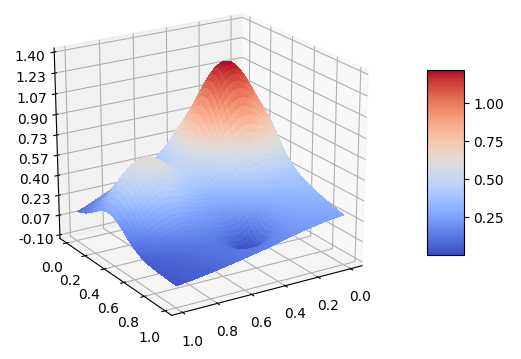
\includegraphics[scale=0.4]{franke.png}
    \caption{Plot of Franke function, with $x,y \in [0,1]$.}
\end{figure}
\section{Results \& Discussion}
Starting with testing an Ordinary Least Squares (OLS) fit to the Franke function. Measuring the MSE and $R^{2}$-score for both the training and test set. By plotting the error measurements as function of the complexity of the model, we can see the effect of increasing the degree of polynomial in our design matrix $\X$. In addition testing for the effect of noise in the dataset, as well as the size of the dataset.
\begin{figure}[ht]
    \centering
    \begin{subfigure}[b]{0.9\columnwidth}
        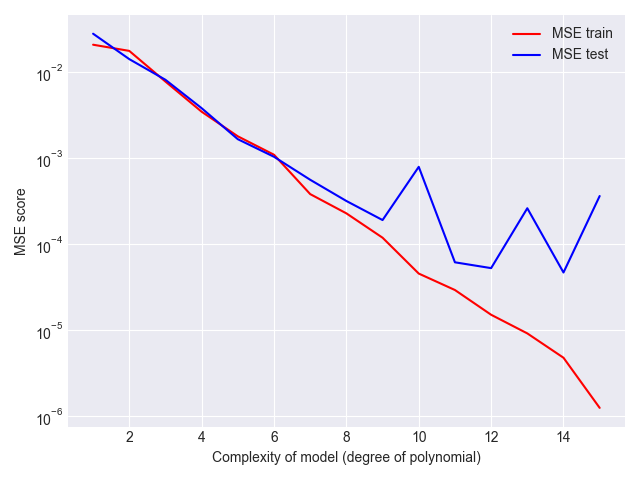
\includegraphics[width=\columnwidth]{mse_vs_complexity_N=400_Noise=0.0_Degree=1-15.png}
        \caption{MSE score for training set and test set with $N = 400$, noise $= 0.0$ and polynomial degrees $1-15$. Y-axis is logarithmically scaled.}
    \end{subfigure}
    
    \begin{subfigure}[b]{0.9\columnwidth}
        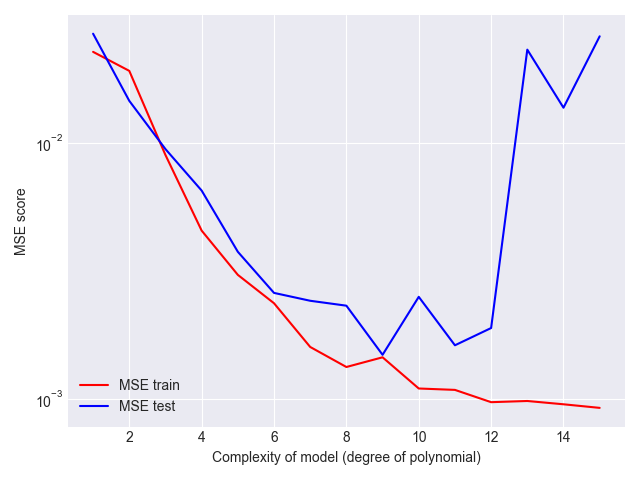
\includegraphics[width=\columnwidth]{mse_vs_complexity_N=400_Noise=0.04_Degree=1-15.png}
        \caption{MSE score for training set and test set with $N = 400$, noise $= 0.04$ and polynomial degrees $1-15$. Y-axis is logarithmically scaled.}
    \end{subfigure}
    \caption{2(a) and 2(b) illustrates the MSE score for each level of complexity. (a) has no added noise to the dataset, while (b) has added noise of 0.04. Score for the test set is plotted in blue and score for training set is plotted in red.}
\end{figure}\\
\noindent Comparing Figure 2(a) and 2(b), we see the effect of noise in our dataset. When noise is added the MSE test starts to rise and gets significantly worse. While the MSE for the training set continuously sinks. Still we see that regardless of if there is noise, that MSE test and train diverges for higher levels of complexity. The reason for this is overfitting. For $N=400$, our model does not generalize enough and therefore fails when new and unseen data is tested on the model.\\
\\
Plotting the $R^{2}$-score for the training set and test set results in Figure 3(a) and 3(b).
\begin{figure}[ht]
    \centering
    \begin{subfigure}[b]{0.9\columnwidth}
        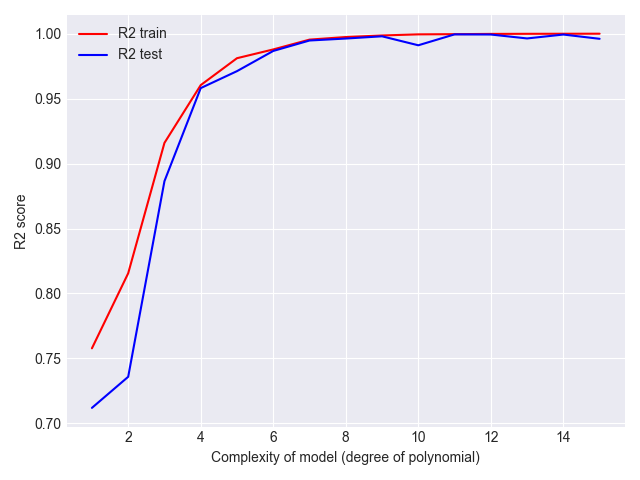
\includegraphics[width=\columnwidth]{r2_vs_complexity_N=400_Noise=0.0_Degree=1-15.png}
        \caption{$R^{2}$-score for training set and test set with $N = 400$, noise $= 0.0$ and polynomial degrees $1-15$. Y-axis is logarithmically scaled.}
    \end{subfigure}
    
    \begin{subfigure}[b]{0.9\columnwidth}
        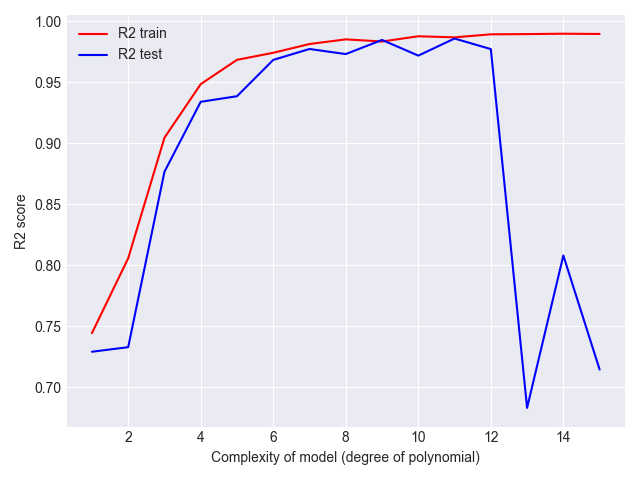
\includegraphics[width=\columnwidth]{r2_vs_complexity_N=400_Noise=0.04_Degree=1-15.png}
        \caption{$R^{2}$-score for training set and test set with $N = 400$, noise $= 0.04$ and polynomial degrees $1-15$. Y-axis is logarithmically scaled.}
    \end{subfigure}
    \caption{3(a) and 3(b) illustrates the $R^{2}$-score for each level of complexity. (a) has no added noise to the dataset, while (b) has added noise of 0.04. Score for the test set is plotted in blue and score for training set is plotted in red.}
\end{figure}\\
\noindent However when comparing Figure 2(a) and Figure 3(a) where no noise is added, we see that the $R^{2}$-score for the test set shows an almost perfect fit for all complexities as opposed to the diverging MSE scores.\ Therefore the $R^{2}$-score may be unreliable when the model is overfitted. If we also compare Figure 2(b) and Figure 3(b) where noise is added, there is more coherence between the MSE and $R^{2}$-score. The MSE and  $R^{2}$-score for the test set are inverse of each other which is what you would expect.
\begin{figure}[ht]
    \centering
    \begin{subfigure}[b]{0.9\columnwidth}
        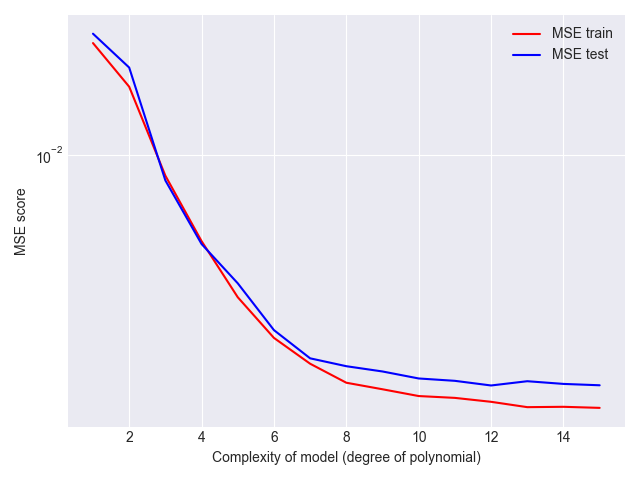
\includegraphics[width=\columnwidth]{mse_vs_complexity_N=2000_Noise=0.04_Degree=1-15.png}
        \caption{MSE score for training set and test set with $N = 2000$, noise $= 0.04$ and polynomial degrees $1-15$. Y-axis is logarithmically scaled.}
    \end{subfigure}
    
    \begin{subfigure}[b]{0.9\columnwidth}
        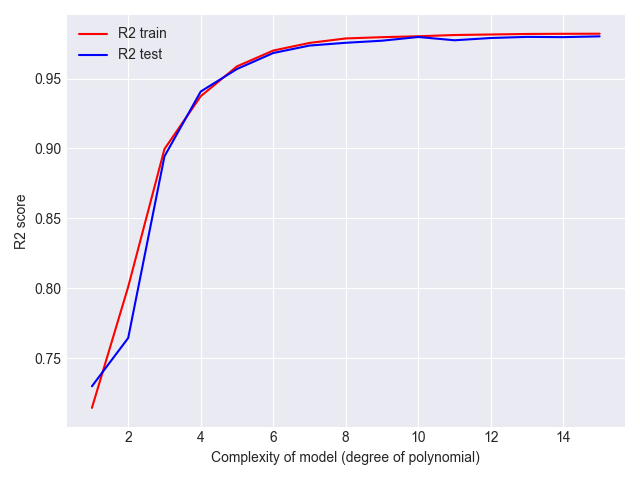
\includegraphics[width=\columnwidth]{r2_vs_complexity_N=2000_Noise=0.04_Degree=1-15.png}
        \caption{$R^{2}$-score for training set and test set with $N = 2000$, noise $= 0.04$ and polynomial degrees $1-15$. Y-axis is logarithmically scaled.}
    \end{subfigure}
    \caption{4(a) and 4(b) plots the MSE and $R^{2}$-score respectively, for each level of complexity. Both scores are calculated from datasets with $N= 2000$ and added noise of 0.04. MSE and $R^{2}$ test is plotted in blue and train is plotted in red.}
\end{figure}\\
In addition to studying the effect of noise, we can study the effect of having a larger dataset. Comparing Figures 4(a) and 4(b) with 2(b) and 3(b), which are plots with the same amount of noise added but the latter has far fewer datapoints. The $R^{2}$ score from 4(b) shows a near perfect fit and the MSE from 4(a) does not contain the large divergence between the MSE train and MSE test that 2(b) does.\\
\\
A larger dataset seems to equalize the effect of noise, and make the model more robust. A robust model will have more accurate $\B$ coefficients. A way to visualize this is to look at the confidence intervals of the variance of the $\B$ coefficients.
\begin{figure}[ht]
    \centering
    \begin{subfigure}[b]{0.9\columnwidth}
        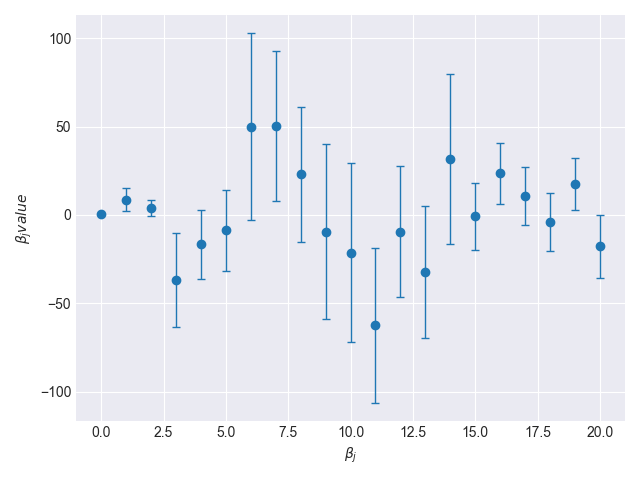
\includegraphics[width=\columnwidth]{conf_intervals_beta_N=400_Noise=0.04_Degree=5.png}
        \caption{Confidence intervals of the individual $\beta_{j}$ for $N = 400$, noise $= 0.04$ and polynomial degree $= 5$. Y-axis shows the actual $\beta_{j}$-values. The errorbar shows the confidence interval.}
    \end{subfigure}
    
    \begin{subfigure}[b]{0.9\columnwidth}
        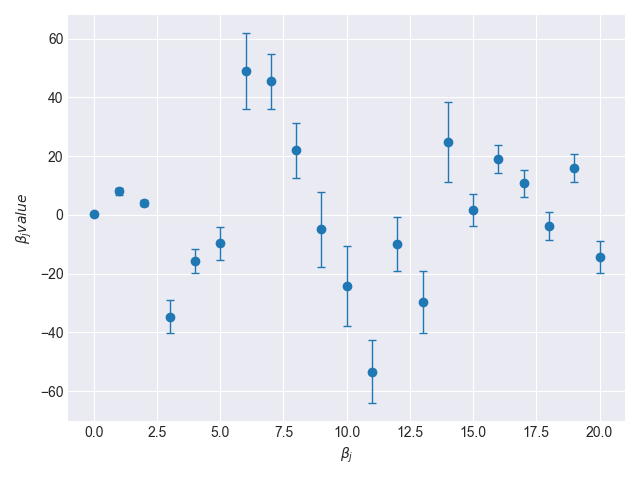
\includegraphics[width=\columnwidth]{conf_intervals_beta_N=2000_Noise=0.04_Degree=5.png}
        \caption{Confidence intervals of the individual $\beta_{j}$ for $N = 2000$, noise $= 0.04$ and polynomial degree $= 5$. Y-axis shows the actual $\beta_{j}$-values.The errorbar shows the confidence interval.}
    \end{subfigure}
    \caption{5(a) and 5(b) visualizes the $95\%$ confidence interval of each $\beta_{j}$ with polynomial degree $= 5$. The confidence interval is given by $\beta_{j} \pm 1.96\overline{\sigma}$, where $\overline{\sigma}$ is the standard deviation of $\beta_{j}$.}
\end{figure}\\
Considering the Figures 5(a) and 5(b), it is evident that having a larger dataset will improve the certainty of the $\B$ coefficients and consequently the accuracy of the model. The confidence intervals are significantly larger for a smaller dataset than a larger dataset.\\
Additionally we study the MSE with the resampling techniques, bootstrap and k-fold cross validation. Comparing the two in 6(a) and 6(b), it is clear that the bootstrap method is more sensitive to noise than k-fold cross validation, and also less stable for higher polynomial degrees. Studying 6(a), the MSE test score with bootstrap starts to become unstable at around polynomial degree 8 and up, whereas with k-fold cross validation it continues to decrease even for higher level of complexity.
\begin{figure}[ht]
    \centering
    \begin{subfigure}[b]{0.9\columnwidth}
        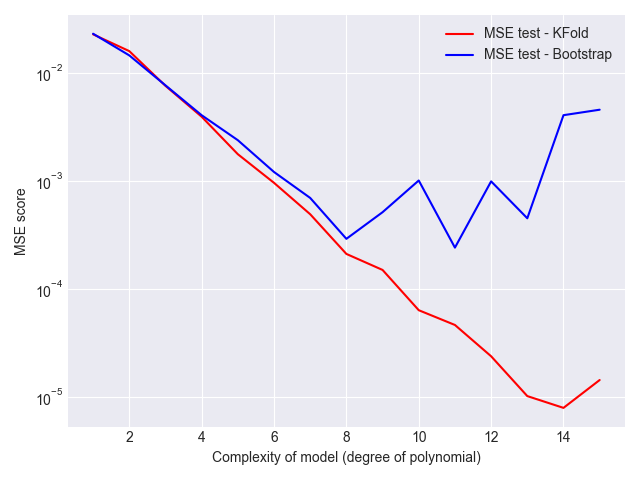
\includegraphics[width=\columnwidth]{kfold_vs_bootstrap_Bootstraps=50,KFolds=10_N=600_Noise=0.0_Degree=1-15.png}
        \caption{MSE test scores for each resampling technique with $N = 600$, noise $= 0.0$, polynomial degrees $1- 15$, bootstraps $= 50$ and k-folds $= 10$. Y-axis is scaled logarithmically.}
    \end{subfigure}
    
    \begin{subfigure}[b]{0.9\columnwidth}
        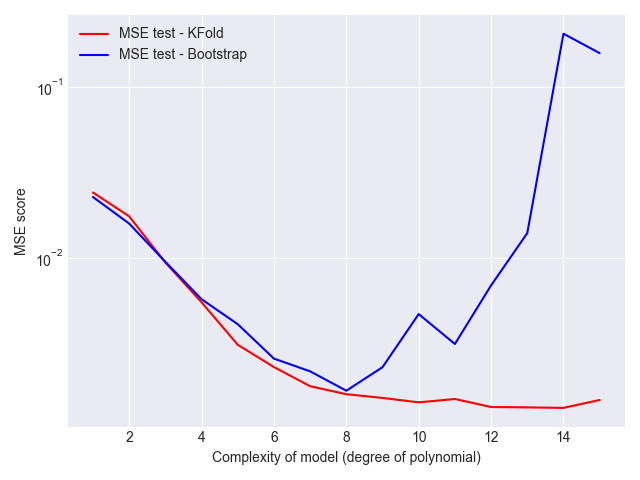
\includegraphics[width=\columnwidth]{kfold_vs_bootstrap_Bootstraps=50,KFolds=10_N=600_Noise=0.04_Degree=1-15.png}
        \caption{MSE test scores for each resampling technique with $N = 600$, noise $= 0.04$, polynomial degrees $1- 15$, bootstraps $= 50$ and k-folds $= 10$. Y-axis is scaled logarithmically}
    \end{subfigure}
    \caption{6(a) and 6(b) plots the MSE test score of each resampling technique with k-folds = $=10$ and bootstraps $= 50$. K-fold cross validation is plotted in red, and bootstrap is blue.}
\end{figure}\\
Studying 6(b), the combination of noise and higher level complexity makes the boostrap method even more unstable and sensitive. Result in almost the same MSE test values when compared to Figure 2(b) where no resampling technique has been used. While minimum for both 2(b) and 6(b) is at polynomial degree 9 and 8 respectively there are no noticeable difference in the MSE score at this level of complexity. \\
\\
Even if for k-fold cross validation the minimum with noise and without noise is at polynomial degree 14, one should be careful not to jump straight to conclusion. While the results with k-fold cross validation are more stable and achieves a lower MSE score, k-fold cross validation may give a too "optimistic" or biased estimate leading to a overfitted model selection\cite{kfold1, kfold2}. However k-fold cross validation is generally more used and provides better results than bootstrap.\\
\\
Continuing with OLS and the bootstrap method to fit the model, we study the bias-variance tradeoff presented previously in section 2.6.2. From Figure 7(a) we see the described effect of high bias, low variance for lower complexity and low bias, high variance for higher complexity. Since the Error = $\textrm{Bias}^{2}$ + Variance + irreducible error, it is to be expected that for lower complexities the bias contributes most to the error because the model is too simple. Also when the model complexity increases we see the bias decreasing steadily towards 0, while the variance increases and starts to contribute more to the error than the bias for higher complexity.\\
\begin{figure}[ht]
    \centering
    \begin{subfigure}[b]{0.9\columnwidth}
        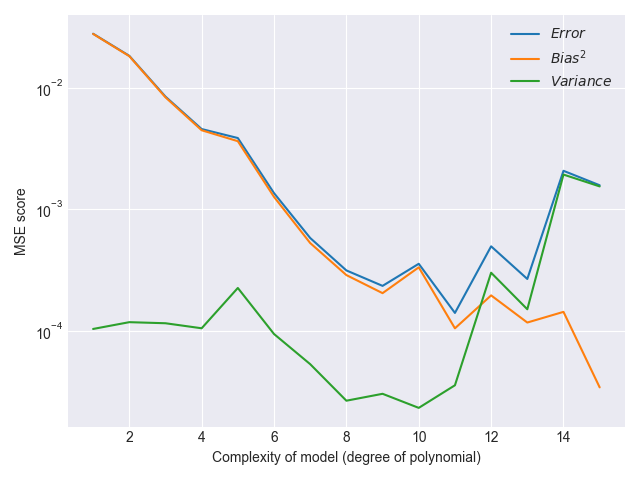
\includegraphics[width=\columnwidth]{bias_variance_tradeoff_Bootstraps=50_N=1000_Noise=0.0_Degree=1-15.png}
        \caption{Bias-variance decomposition for $N = 1000$, noise $= 0.0$, polynomial degrees $1- 15$ and bootstraps $= 50$. Y-axis is scaled logarithmically.}
    \end{subfigure}
    
    \begin{subfigure}[b]{0.9\columnwidth}
        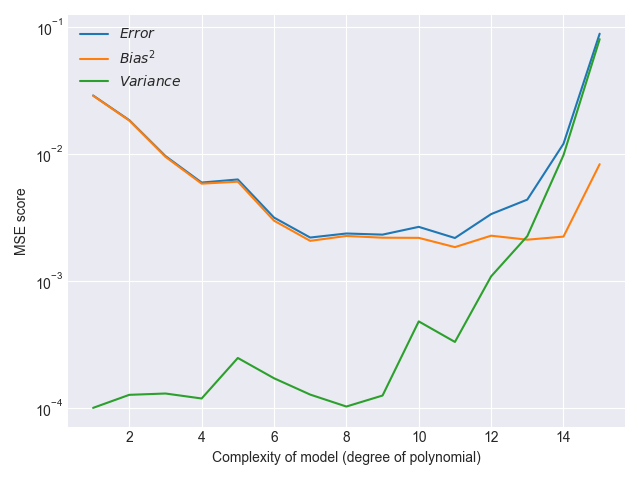
\includegraphics[width=\columnwidth]{bias_variance_tradeoff_Bootstraps=50_N=1000_Noise=0.04_Degree=1-15.png}
        \caption{Bias-variance decomposition for $N = 1000$, noise $= 0.04$, polynomial degrees $1- 15$ and bootstraps $= 50$. Y-axis is scaled logarithmically.}
    \end{subfigure}
    \caption{7(a) and 7(b) plots the bias-variance decomposition for the MSE test score with OLS. For both figures, the bootstrap method was used as the resampling technique, with bootstraps $= 50$. The MSE is plotted in blue, bias in orange and the variance in green. }
\end{figure}\\
Using the OLS estimator, the test error has a minimum for polynomial degree 11. Polynomial degree 11 is the optimal level of complexity for the model fitted to the specific dataset. This where there is a balance between the variance and bias, and neither overpowers the other. \\
\\
On the other hand, from Figure 7(b) we see that with noise the optimal level of complexity is approximately polynomial degree 7 but we could choose a complexity between 7-11 seeing as the error is almost constant in the interval. The error is higher compared to (a) beacause of the added noise, but the model has a lower level of complexity. It is preferable to have a lower complexity because we need fewer $\B$ coefficients to sufficiently fit the model to the dataset.\\
Unlike the bias in Figure 7(a), the bias in Figure 7(b) does not continue decreasing towards 0 like expected. Instead the bias flattens out and remains almost constant from polynomial degree 7 and up until it increases. The reason for this may be numerical instability, but the instability could also be caused by the high degree of polynomial. It may be the case that the model can sufficiently fit to the Franke function with a lower degree of polynomial, but as the complexity is increased it "blows up" the values to a point where the model can no longer be fitted accurately and therefore introducing bias.\\
\\
Now we introduce Ridge regression and Lasso regression to study the effect of a regularization parameter on the bias-variance. Figure 8 show the plot of the bias-variance decomposition with Ridge regression for $\lambda = 1\textrm{e}-10$.
\begin{figure}[ht]
    \centering
    \begin{subfigure}[b]{0.9\columnwidth}
        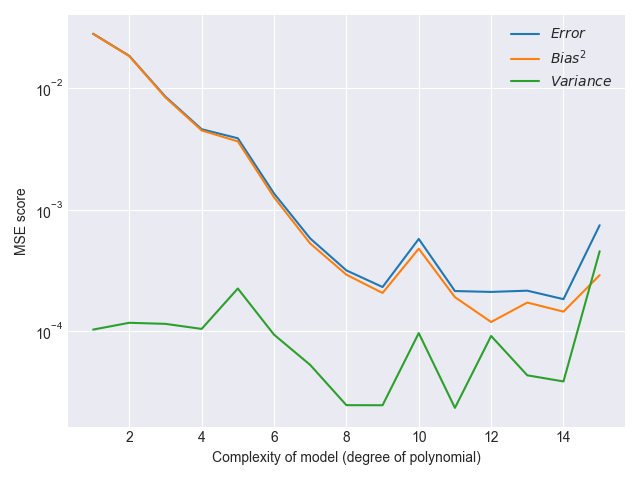
\includegraphics[width=\columnwidth]{bias_variance_tradeoff_Lambda=1e-10_Bootstraps=50_N=1000_Noise=0.0_Degree=1-15.png}
        \caption{Bias-variance decomposition for $N = 1000$, noise $= 0.0$, polynomial degrees $1- 15$ and bootstraps $= 50$. The regularization parameter is set to $\lambda = 1\textrm{e}-10$. Y-axis is scaled logarithmically.}
    \end{subfigure}
    
    \begin{subfigure}[b]{0.9\columnwidth}
        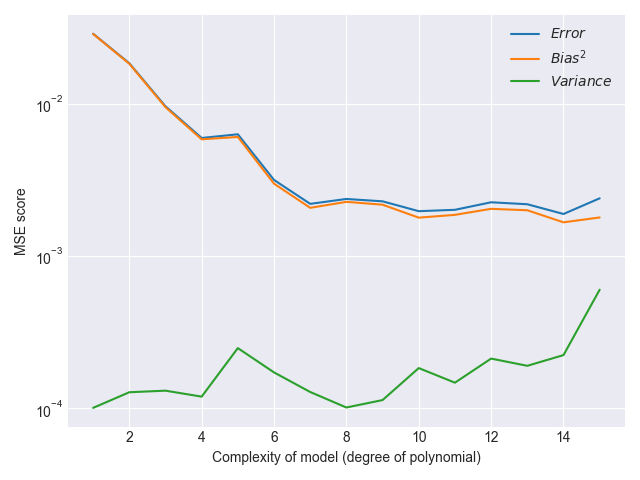
\includegraphics[width=\columnwidth]{bias_variance_tradeoff_Lambda=1e-10_Bootstraps=50_N=1000_Noise=0.04_Degree=1-15.png}
        \caption{Bias-variance decomposition for $N = 1000$, noise $= 0.04$, polynomial degrees $1- 15$ and bootstraps $= 50$. The regularization parameter is set to $\lambda = 1\textrm{e}-10$. Y-axis is scaled logarithmically.}
    \end{subfigure}
    \caption{8(a) and 8(b) plots the bias-variance decomposition for the MSE test score with Ridge regression. For both figures, the bootstrap method was used as the resampling technique, with bootstraps $= 50$ and $\lambda = 1\textrm{e}-10$.. The MSE is plotted in blue, bias in orange and the variance in green. }
\end{figure}\\
Comparing the bias-variance for OLS and Ridge regression, we see that the variance when using Ridge regression does not start to increase until around polynomial degree 14 unlike with OLS where the variance increases at degree 9 or 10. Figure 8(a) shows that the variance does not overpower the bias until polynomial degree 15 and in 8(b) the bias overpowers the variance for all polynomial degrees 1-15. Also comparing 7(b) and 8(b), the error at the minimum is almost the same but as the complexity increases Ridge remains relatively stable while the error with OLS asymptotically increases.
\begin{figure}[ht]
    \centering
    \begin{subfigure}[b]{0.9\columnwidth}
        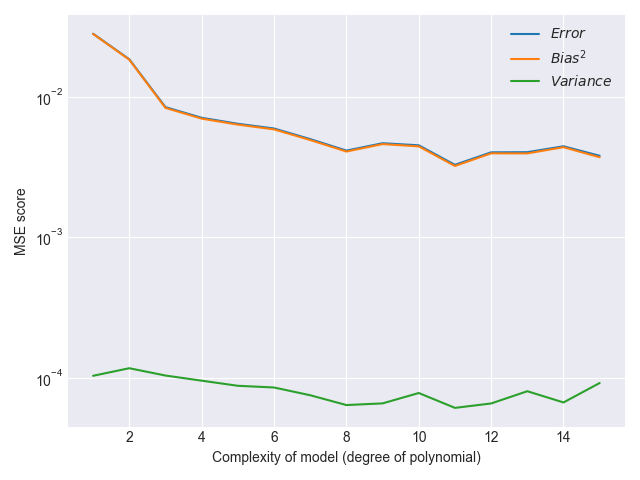
\includegraphics[width=\columnwidth]{bias_variance_tradeoff_Lambda=0.01_Bootstraps=50_N=1000_Noise=0.0_Degree=1-15.png}
        \caption{Bias-variance decomposition for $N = 1000$, noise $= 0.0$, polynomial degrees $1- 15$ and bootstraps $= 50$. The regularization parameter is set to $\lambda = 1\textrm{e}-2$. Y-axis is scaled logarithmically.}
    \end{subfigure}
    
    \begin{subfigure}[b]{0.9\columnwidth}
        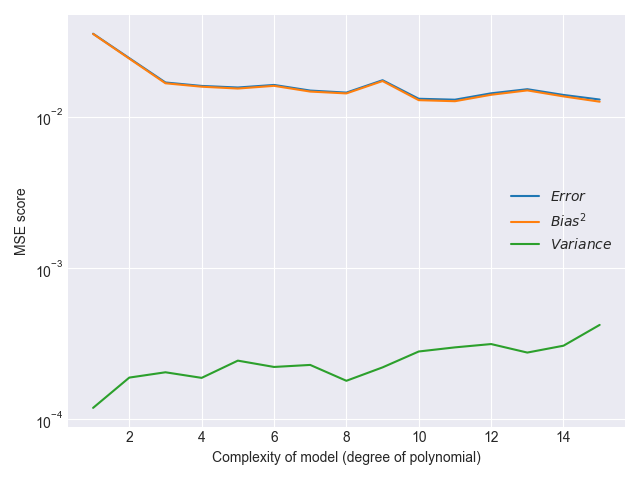
\includegraphics[width=\columnwidth]{bias_variance_tradeoff_Lambda=0.01_Bootstraps=50_N=1000_Noise=0.1_Degree=1-15.png}
        \caption{Bias-variance decomposition for $N = 1000$, noise $= 0.1$, polynomial degrees $1- 15$ and bootstraps $= 50$. The regularization parameter is set to $\lambda = 1\textrm{e}-2$. Y-axis is scaled logarithmically.}
    \end{subfigure}
    \caption{9(a) and 9(b) plots the bias-variance decomposition for the MSE test score with Ridge regression. For both figures, the bootstrap method was used as the resampling technique, with bootstraps $= 50$ and $\lambda = 1\textrm{e}-2$. The MSE is plotted in blue, bias in orange and the variance in green. }
\end{figure}\\
The reason for the difference between OLS and Ridge regression in how the bias and variance behaves is due to the regularization parameter $\lambda$. We explained earlier that the regularization parameter shrinks certain features that are less important. As a result, bias is introduced in the model which reduce the variance. For this reason the MSE does not asymptotically increase for higher complexities like with OLS in Figure 7. \\
\\
After increasing the regularization parameter to $\lambda = 1\textrm{e}-2$, we can more clearly see the effect of varying $\lambda$. Comparing Figure 9 to 8, a higher $\lambda$ adds even more bias and decreases the variance, and therefore keeps the error almost constant when increasing the complexity of the model. In addition to preventing the error from asymptotically increase for higher complexity, Ridge regression also handles noise better than OLS. In Figure 9(b) the noise was more than doubled while keeping the size of the dataset the same. Even though the error at the minimum is higher compared to OLS, the ability of Ridge regression to remain stable for higher complexities when the dataset contains a lot of noise is extremely valuable.\\
\\
Figure 10 shows the bias-variance decomposition of the error using Lasso regression. 
\begin{figure}[ht]
    \centering
    \begin{subfigure}[b]{0.9\columnwidth}
        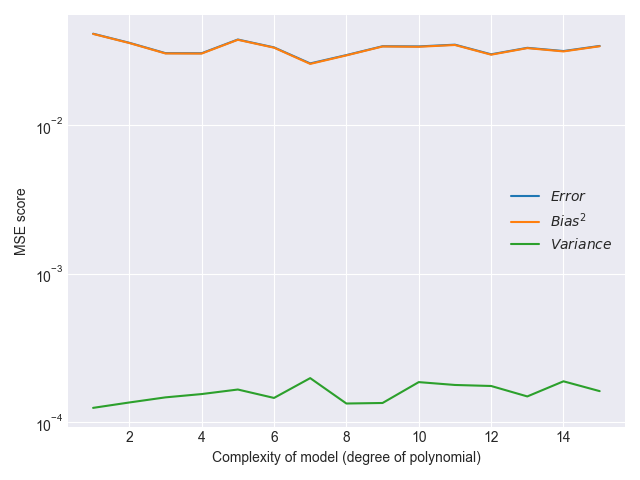
\includegraphics[width=\columnwidth]{bias_variance_tradeoff_lasso_Lambda=0.01_Bootstraps=50_N=1000_Noise=0.1_Degree=1-15.png}
        \caption{Bias-variance decomposition for $N = 1000$, noise $= 0.1$, polynomial degrees $1- 15$ and bootstraps $= 50$. The regularization parameter is set to $\lambda = 1\textrm{e}-2$. Y-axis is scaled logarithmically.}
    \end{subfigure}
    \caption{10(a) plots the bias-variance decomposition for the MSE test score with Lasso regression. The bootstrap method was used as the resampling technique, with bootstraps $= 50$ and $\lambda = 1\textrm{e}-2$. The MSE is plotted in blue, bias in orange and the variance in green. }
\end{figure}\\
With the same size dataset, added noise, and $\lambda$ value, there is no significant difference between Ridge regression in 9(b) and Lasso regression in 10(a). With Lasso regression, the error converges at a slightly higher value compared to with Ridge, but the variance remains more stable for higher complexity. As the complexity increases we see from 9(b) that the variance slowly increases with Ridge regression, compared to an almost constant variance in 10(a) for Lasso regression. This may indicate that Lasso is more robust for high level of complexity and a dataset with a lot of noise.\\
\\
Next we compare all introduced regression methods using k-fold cross validation as the resampling technique.
\begin{figure}[ht]
    \centering
    \begin{subfigure}[b]{0.9\columnwidth}
        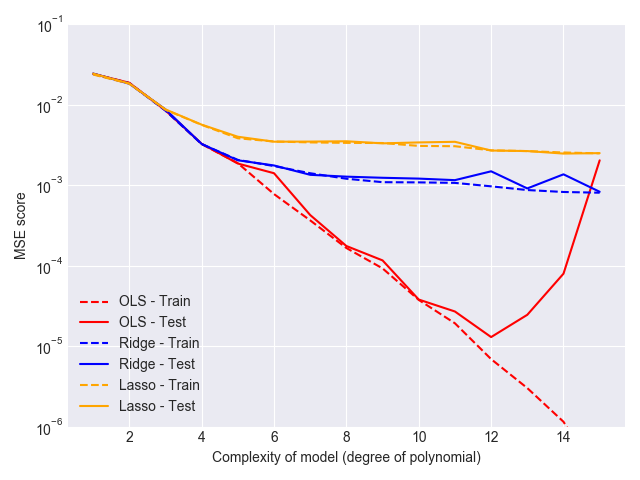
\includegraphics[width=\columnwidth]{OLS_Ridge_Lasso_comparison_Lambda=1e-05_N=200_Noise=0.0_Degree=1-15.png}
        \caption{MSE test and train scores for each regression method with $N = 200$, noise $= 0.0$, polynomial degrees $1- 15$ and k-folds $= 10$. The regularization parameter is set to $\lambda = 1\textrm{e}-5$. Y-axis is scaled logarithmically.}
    \end{subfigure}
    
    \begin{subfigure}[b]{0.9\columnwidth}
        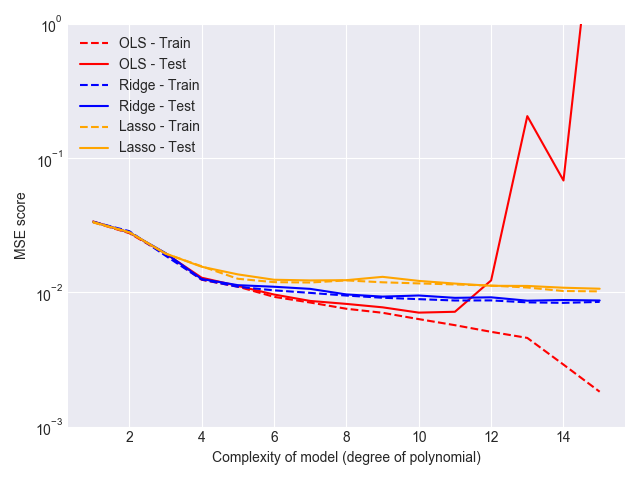
\includegraphics[width=\columnwidth]{OLS_Ridge_Lasso_comparison_Lambda=1e-05_N=200_Noise=0.1_Degree=1-15.png}
        \caption{MSE test and train scores for each regression method with $N = 200$, noise $= 0.1$, polynomial degrees $1- 15$ and k-folds $= 10$. The regularization parameter is set to $\lambda = 1\textrm{e}-5$. Y-axis is scaled logarithmically.}
    \end{subfigure}
    \caption{11(a) and 11(b) compares the MSE score for the training set and test set for each regression method. The MSE train score is plotted as a dotted line, while MSE test score is plotted as a solid line. OLS is plotted in red, Ridge in blue and Lasso in orange. K-fold cross validation was used as the resampling technique.}
\end{figure}\\
Important to note about the results in Figure 11 is the random apsect of the k-fold cross validation algorithm.\ While holding all parameters and dataset constant, the random shuffle of the dataset in the algorithm will result in different MSE scores when the code is run again. Especially for OLS. Still, when run enough times we start to see similar trends.\\
\\
Comparing the regression methods in 11(a) we see that the OLS estimator results in the best fit for polynomial degrees 4 up to around 12. At this point the test error starts to diverge from the train error and asymptotically increase, not unlike we have seen earlier in the results and discussion. Ridge and Lasso converges and the error remains relatively constant as the complexity increases from polynomial degree 6, where Ridge results in a lower error compared to Lasso when no noise is added. Although for higher complexity the Ridge test error varies slightly from the train error compared to Lasso where the test and train error are essentially identical. The slight variation for Ridge may be caused by the numerical instability. \\
\\
Ridge and Lasso results in more stable test errors for higher complexities compared to OLS in both 11(a) and 11(b), which was also discussed when looking at the bias-variance decomposition. The error for OLS with polynomial degrees up to 12 in 11(b) is almost identical to that of Ridge and Lasso regression, where it for higher degrees sharply diverges from the train error due to overfitting and the added noise. When comparing Ridge and Lasso in Figure 11(b), the errors converges at a similar value. This may indicate that Lasso is more robust for smaller datasets with a lot of noise. To further investigate the differences between Ridge and Lasso, we study the effect of varying the regularization paramater $\lambda$ with the heatmaps of Figure 12. The added noise is a high value compared to the size of the dataset. This is done to study which regression method is more robust against noise and a smaller dataset.\\
\\
When comparing 12(a) and 12(b), the $R^{2}$-scores reinforces the results from 11(a) and 11(b) where generally Ridge regression performs better than Lasso regression in achieving a lower error. The heatmaps show Ridge regression generally achieving a better fit for almost all combinations of polynomial degree and $\lambda$. Also with Lasso regression the $R^{2}$-score for higher $\lambda$ values deteriorates faster than with Ridge regression. \\
\\
All in all, the two regression methods achieve fairly similar results on the current dataset. The downside with using Lasso regression is that it is much more computationally expensive compared to Ridge regression, especially for lower $\lambda$ values Lasso requires a high number of iterations to converge. On the other hand, Ridge is limited by not being able to zero out certain features. \\
\begin{figure}[ht]
    \centering
    \begin{subfigure}[b]{0.9\columnwidth}
        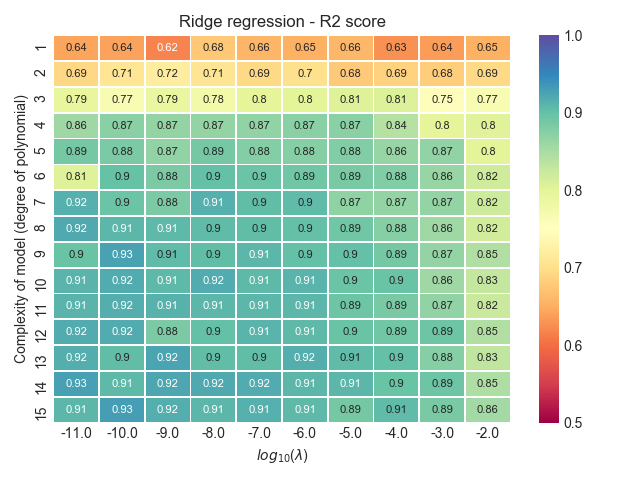
\includegraphics[width=\columnwidth]{lambda_vs_complexity_heatmap_Ridge_N=200_Noise=0.1_Degree=115.png}
        \caption{$R^{2}$-scores for Ridge regression with $N = 200$, noise $= 0.1$, polynomial degrees $1- 15$, $\lambda = [1\textrm{e}-11, 1\textrm{e}-2]$, and k-folds $= 10$.}
    \end{subfigure}
    
    \begin{subfigure}[b]{0.9\columnwidth}
        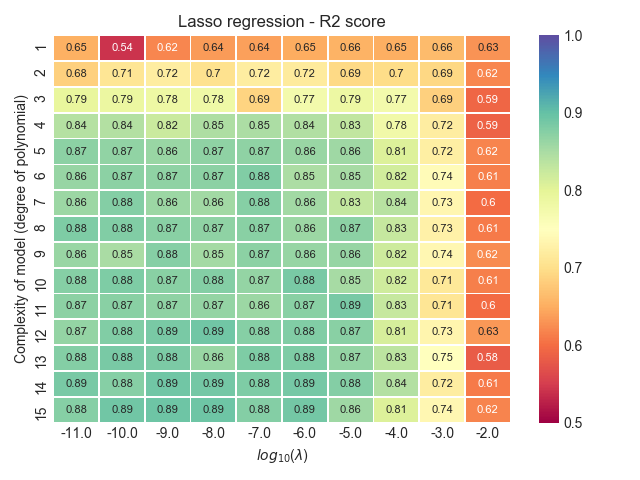
\includegraphics[width=\columnwidth]{lambda_vs_complexity_heatmap_Lasso_N=200_Noise=0.1_Degree=115.png}
        \caption{$R^{2}$-scores for Lasso regression with $N = 200$, noise $= 0.1$, polynomial degrees $1- 15$, $\lambda = [1\textrm{e}-11, 1\textrm{e}-2]$, and k-folds $= 10$.}
    \end{subfigure}
    \caption{12(a) and 12(b) shows the heatmap of the $R^{2}$-score for Ridge and Lasso regression with the Franke function. Colorbar has a minimum value 0.5 and maxiumum value 1. K-fold cross validation was used as the resampling technique.}
\end{figure}\\
But in the case with the Franke function, this may not be important if almost every feature contributes equally. In general it is clear from 12(a) and 12(b) that a lower $\lambda$ value will result in a better fit for both Ridge and Lasso regression. This is logical seeing as when $\lambda$ approaches 0, the estimate approaches the OLS estimate.\\
\\
\noindent Up until now we have tested the different regression methods on the Franke function to see how they differ when varying certain parameters. Now we apply the regression methods on a subset of the real terrain data presented previously.
\begin{figure}[ht]
    \centering
    \begin{subfigure}[b]{0.9\columnwidth}
        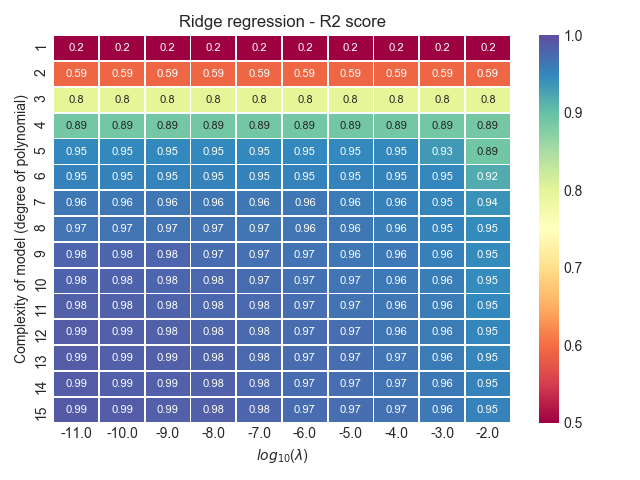
\includegraphics[width=\columnwidth]{lambda_vs_complexity_heatmap_Ridge_N=10000_Noise=0.0_Degree=115.png}
        \caption{$R^{2}$-scores for Ridge with a subset size of $N=10000$ with polynomial degrees $1- 15$, $\lambda = [1\textrm{e}-11, 1\textrm{e}-2]$, and k-folds $= 10$.}
    \end{subfigure}
    
    \begin{subfigure}[b]{0.9\columnwidth}
        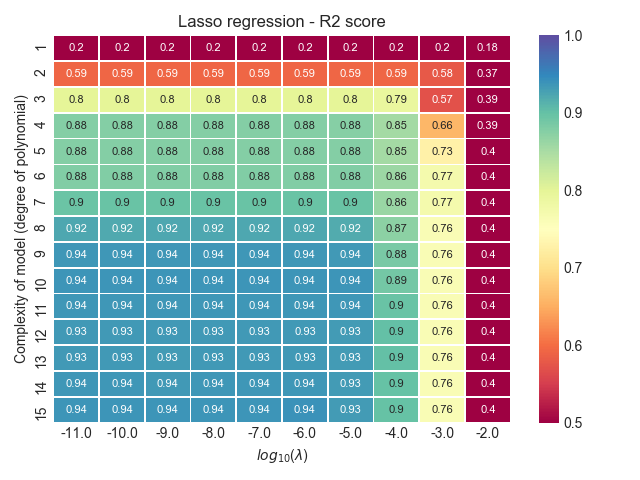
\includegraphics[width=\columnwidth]{lambda_vs_complexity_heatmap_Lasso_N=10000_Noise=0.0_Degree=115.png}
        \caption{$R^{2}$-scores for Lasso with a subset size of $N=10000$ with polynomial degrees $1- 15$, $\lambda = [1\textrm{e}-11, 1\textrm{e}-2]$, and k-folds $= 10$.}
    \end{subfigure}
    \caption{13(a) and 13(b) shows the heatmap of the $R^{2}$-score for Ridge and Lasso regression with a subset of the terrain data. Colorbar has a minimum value 0.5 and maxiumum value 1. K-fold cross validation was used as the resampling technique.}
\end{figure}\\
From Figure 13(a), the best fit with Ridge regession is $R^{2}=0.99$ for polynomial degree 12 and $\lambda = 1\textrm{e}-11$. While the best fit with Lasso regression is $R^{2} = 0.94$ for polynomial degree 9 and $\lambda = 1\textrm{e}-11$. \\
\\
Generally Ridge regression achieves a much better fit for polynomial degrees 4 and higher, and also is more stable for all $\lambda$ values tested. An important note is that Lasso regression may perform better for higher complexities but due to the iterative algorithm of Lasso regression we are unable to test because it will take to much time computationally.\\
\\
However given the nature of the dataset and the way the design matrix is structured with increasing degrees of polynomials as columns, it makes sense that most of the features will contribute to the modeling of the terrain to a certain point. Due to this, the advantage of using Lasso with the ability to set certain $\B$ coefficients to 0, becomes insignificant. Therefore it is not unusual that Ridge regression generally fits better than Lasso regression for the terrain data.\\
\\ 
Now that we have found the best $\lambda$ values to use with Ridge and Lasso regression, we can compare all the regression methods.\\
\\
As we can see from Figure 14, OLS results in the best MSE score with Ridge regression at a close second and Lasso regression performing worst of the three regression methods. This result for the terrain data support the results with the Franke function. We could not test Lasso regression for more than polynomial degree 20 because it would take too much time. Table 1 shows the minimum for each regression method.\\
\begin{table}[h]
    \centering
    \caption{Minimum MSE test scores from Figure 14. K-fold cross validation used as resampling technique with k-folds $= 10$.}
    \begin{tabular}{|c||c|c|c|c| }
    \hline
        Method & Degree & $\lambda$ & $R^{2}$ & MSE test \\ 
        \hline\hline
        OLS & 30 & - & $0.99$ & $0.00024$ \\ 
        \hline
        Ridge & 27 & $1\textrm{e}-11$ & $0.99$ & $0.00094$ \\
        \hline
        Lasso & 19 & $1\textrm{e}-11$ & $0.94$ & $0.00641$\\
        \hline
    \end{tabular}
\end{table}
\begin{figure}[H]
    \centering
    \begin{subfigure}[b]{0.9\columnwidth}
        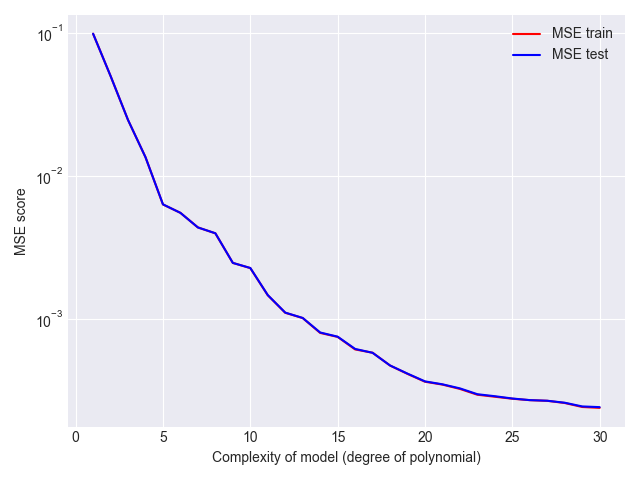
\includegraphics[width=\columnwidth]{mse_vs_complexity_OLS_N=10000_Noise=0.0_Degree=1-30.png}
        \caption{MSE-scores for OLS fitted to the terrain where $N = 10000$, and for polynomial degrees $1- 30$ and kfolds $= 10$. Y-axis is scaled logarithmically.}
    \end{subfigure}
    
    \begin{subfigure}[b]{0.9\columnwidth}
        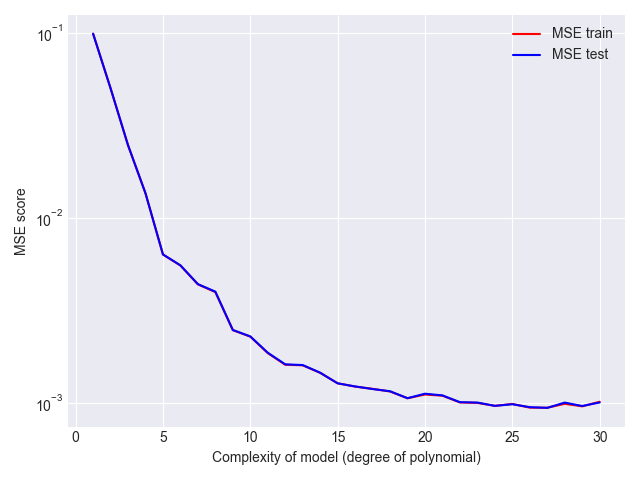
\includegraphics[width=\columnwidth]{mse_vs_complexity_Ridge_N=10000_Noise=0.0_Degree=1-30.png}
        \caption{MSE-scores for Ridge fitted to the terrain where $N = 10000$, and for polynomial degrees $1- 30$ and kfolds $= 10$. The regularization parameter is set to $\lambda = 1\textrm{e}-11$. Y-axis is scaled logarithmically.}
    \end{subfigure}
    
    \begin{subfigure}[b]{0.9\columnwidth}
        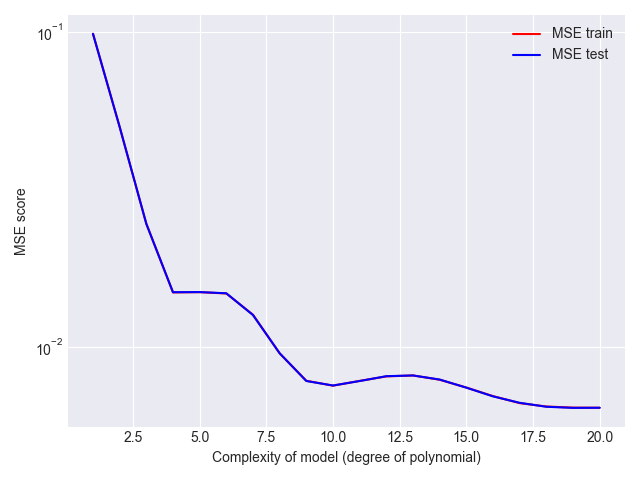
\includegraphics[width=\columnwidth]{mse_vs_complexity_Lasso_N=10000_Noise=0.0_Degree=1-20.png}
        \caption{MSE-scores for Lasso fitted to the terrain where $N = 10000$, and for polynomial degrees $1- 20$ and kfolds $= 10$. The regularization parameter is set to $\lambda = 1\textrm{e}-11$. Y-axis is scaled logarithmically.}
    \end{subfigure}
    \caption{Plots the error for the different regression methods fitted to the terrain with k-fold cross validation as resampling technique. The test error is plotted in blue, and the train error in red.}
\end{figure}\\
\noindent From the results of Figure 14, it is evident that a higher level of complexity is necessary to model the terrain data compared to the Franke function. OLS and Ridge regression both reaches a minimum at a very high complexity, and while we could not test Lasso with a higher complexity we see that Lasso starts to converge already at polynomial degree 18. To test if Lasso remains relatively constant for higher complexities, Lasso was tested with the same parameters except increasing the polynomial degree to 27. Table 2 shows the result. As we see from the results, the error for Lasso converges at almost the exact value as in Table 1 and remains constant for higher complexity.
\begin{table}[h]
    \centering
    \caption{Lasso regression with polynomial degree 27. K-fold cross validation used as resampling technique with k-folds $= 10$.}
    \begin{tabular}{|c||c|c|c|c| }
    \hline
        Method & Degree & $\lambda$ & $R^{2}$ & MSE test \\ 
        \hline\hline
        Lasso & 27 & $1\textrm{e}-11$ & $0.94$ & $0.00655$\\
        \hline
    \end{tabular}
\end{table}\\
Using OLS with a high level of complexity results in the best fit and error scores on the terrain data. The reason why we do not see a large divergence between the MSE test and train scores is because the terrain data does not contain any decisive noise. If the data did contain a lot of noise, it is not unlikely we would see Ridge regression and Lasso regression performing better than OLS for higher polynomial degrees due to the variance "blowing up".\\
\\
We see from Figure 15(a) with OLS that the bias-variance decomposition for the terrain data is dominated by the bias for all polynomial degrees. Therefore the usefulness and necessity of a regularization parameter $\lambda$ like with Ridge and Lasso regression is reduced. While error with OLS is more unstable for higher complexity in 15(a), the error is still lower than with Ridge and Lasso in 15(b) and 15(c) respectively. \\
\\
Again we see also see the difference in result between Ridge and Lasso regression in 15(b) and 15(c). The error for Ridge converges at a lower value than Lasso, but the variance remains relatively constant at a similar value.\\
\\
\begin{figure}[ht]
    \begin{subfigure}{0.475\columnwidth}
        \centering
        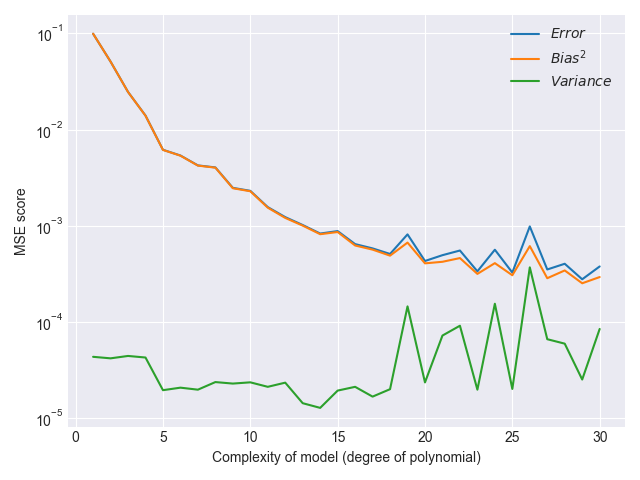
\includegraphics[width=\columnwidth]{bias_variance_tradeoff_OLS_Bootstraps=50_N=10000_Noise=0.0_Degree=1-30.png}
        \caption{Bias-variance decomposition with OLS for $N=10000$ and polynomial degrees $1-30$.}
    \end{subfigure}\hspace{0.1cm}
    \begin{subfigure}{0.475\columnwidth}
        \centering
        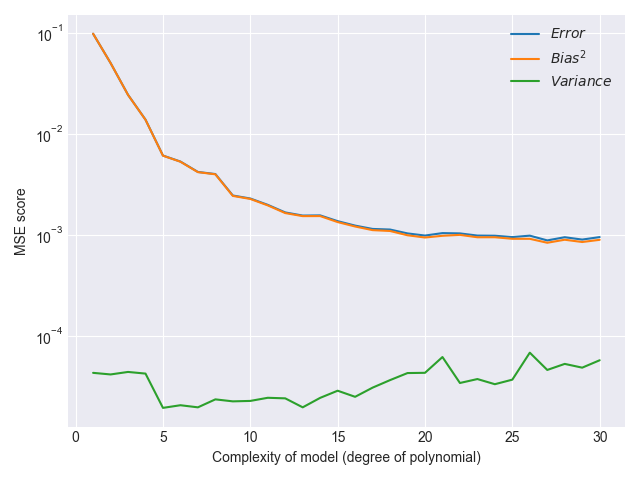
\includegraphics[width=\columnwidth]{bias_variance_tradeoff_Ridge_Lambda=1e-11_Bootstraps=50_N=10000_Noise=0.0_Degree=1-30.png}
        \caption{Bias-variance decompositon with Ridge for $N=10000$, polynomial degrees $1-30$ and $\lambda = 1\textrm{e}-11$.}
    \end{subfigure}\\[1ex]
    \centering
    \begin{subfigure}{0.5\columnwidth}
        \centering
        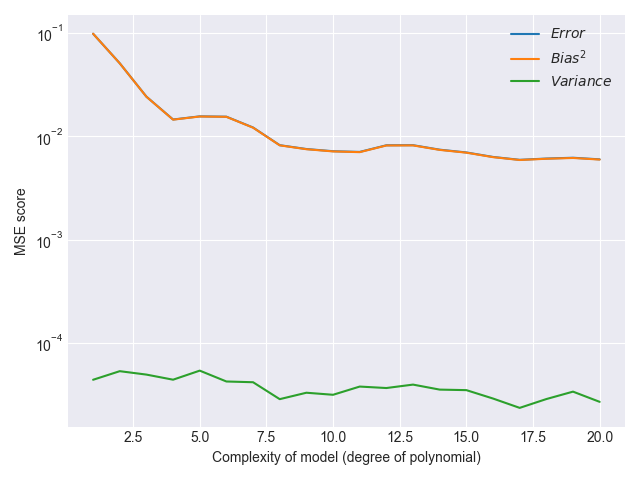
\includegraphics[width=\columnwidth]{bias_variance_tradeoff_Lasso_Lambda=1e-11_Bootstraps=50_N=10000_Noise=0.0_Degree=1-20.png}
        \caption{Bias-variance decompositon with Lasso for $N=10000$, polynomial degrees $1-20$, and $\lambda = 1\textrm{e}-11$.}
    \end{subfigure}
    \caption{Bias-variance decomposition with OLS, Ridge and Lasso. Bootstrap method was used as resampling technique with bootstraps $=50$.}
\end{figure}\\
Figure 16 below shows the predicted terrain with each regression method compared with the actual terrain. The result is in effect just a confirmation of the previous results. The predicted terrain with OLS captures more details, especially the differences in the higher(lighter) regions. Ridge performs relatively well but the terrain is more smoothed out than with OLS. The predicted terrain with Lasso is even more smoothed out and not a lot of the finer details of the actual terrain remains.
\begin{figure*}
    \centering
    \begin{subfigure}[b]{0.5\columnwidth}
        
\includegraphics[width=\columnwidth]{terrain_subset.png}
        \caption{Actual terrain}
    \end{subfigure}\hspace{0.2cm}
    \begin{subfigure}[b]{0.5\columnwidth}
        
\includegraphics[width=\columnwidth]{terrain_predict.png}
        \caption{OLS}
    \end{subfigure}
    \vskip\baselineskip
    \begin{subfigure}[b]{0.5\columnwidth}
        
\includegraphics[width=\columnwidth]{terrain_predict_Ridge.png}
        \caption{Ridge regression}
    \end{subfigure}\hspace{0.2cm}
    \begin{subfigure}[b]{0.5\columnwidth}
        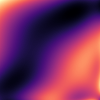
\includegraphics[width=\columnwidth]{terrain_predict_Lasso.png}
        \caption{Lasso regression}
    \end{subfigure}
    \captionsetup{width=1.5\columnwidth}
    \caption{Comparison of the actual terrain data with the predicted terrain using OLS, Ridge regression and Lasso regression.}
\end{figure*}\\
\newpage
\section{Conclusion}
The performance of OLS, Ridge and Lasso, when tested on the Franke function, was found to be dependent on the size of the dataset, the amount of noise and the level of complexity. A large dataset with no noise favored OLS, but for a smaller dataset or with noise OLS tended to overfit for higher complexity because the variance dominated the bias.\\
\\
Ridge and Lasso was found to be more favored for smaller datasets and datasets with noise. Both regression methods contains a regularization parameter which resulted in a slightly higher error, but a more robust and stable performance compared to OLS when noise is added and for higher complexity. To explain why, we looked at the bias-variance tradeoff and the plotted decomposition of the error. The regularization parameter $\lambda$ increased bias which reduced the variance, and the error usually converged for higher complexity. Generally Ridge performed noticeably better than Lasso in every instance.\\
\\
When comparing the resampling methods used in the project, k-fold cross validation provided more stable and better results than the bootstrap method. The bootstrap method was found to be more sensitive to noise and also performs worse for higher complexity. However k-fold cross validation may provide a too "optimistic" result which may lead to selecting a overfitted model during model selection if you are not careful.\\
\\
Applying the regression methods on the terrain data, using k-fold cross validation, resulted in much of the same results as when tested on the Franke function. OLS performed best on the terrain data due to the large dataset and no noise in the dataset. Ridge performed slighlty worse than OLS, but the error estimate was more stable with Ridge for higher complexity. Lasso did not perform as well as OLS and Ridge and converged on a higher error. Due to the nature of the terrain data, the regularization parameter $\lambda$ for Ridge and Lasso regression proved to be insignificant and inconsequential. 
\begin{thebibliography}{9}
\bibitem{epidemiology}
Bender, R. (2009). Introduction to the use of regression models in epidemiology. Methods in molecular biology (Clifton, N.J.), 471, 179–195. \url{https://pubmed.ncbi.nlm.nih.gov/19109780/}

\bibitem{ridge1}
van Wieringen, W.N. (2020). Lecture notes on ridge regression. \url{https://arxiv.org/pdf/1509.09169.pdf}

\bibitem{ridge2}
Hastie, T. et al. (2017). The Elements of Statistical Learning, Second Edition. Springer. 

\bibitem{linalg}
Lay, David C. et al. (2018). Linear Algebra and its Applications, Global Edition. Pearson. 

\bibitem{kfold1}
Bengio, Y. \& Grandvalet, Y. (2004). No Unbiased Estimator of the Variance of K-Fold Cross Validation. Journal of Machine Learning Research, 5. \url{https://www.jmlr.org/papers/volume5/grandvalet04a/grandvalet04a.pdf}

\bibitem{kfold2}
Cawley, G.C. \& Talbot, N.L.C. (2010). On Over-fitting in Model Selection and Subsequent Selection Bias in Performance Evaluation. Journal of Machine Learning Research, 11. \url{https://jmlr.csail.mit.edu/papers/volume11/cawley10a/cawley10a.pdf}
\end{thebibliography}
\newpage
\begin{appendices}
\section{Bias-variance decomposition}\label{app:A}
Decomposition of MSE
\begin{align*}
    \E[(\y - \ytilde)^{2}] &= \E[(f + \mathbf{\epsilon} 
    - \ytilde)^{2}]\numberthis\label{eqn}\\
    &=\E[\left(f + \mathbf{\epsilon} - \ytilde + \E[\ytilde] - \E[\ytilde]\right)^{2}]\numberthis\label{eqn}\\
    &= \E[(f - \E[\ytilde])^{2}] + \E[\mathbf{\epsilon}^{2}]\\ &\hspace{0.4cm}+ \E[(\E[\ytilde] - \ytilde)^{2}]\\
    &\hspace{0.4cm}+ 2(f - \E[\ytilde])]\E[\mathbf{\epsilon}] \\
    &\hspace{0.4cm}+ 2\E[(\E[\ytilde] - \ytilde)]\E[\mathbf{\epsilon}] \\
    &\hspace{0.4cm}+ 2(f - \E[\ytilde])\E[(\E[\ytilde]-\ytilde)]\numberthis\label{eqn}\\
    &= \E[(f-\E[\ytilde])^{2} + \mathbf{\epsilon}^{2} + (\E[\ytilde] - \ytilde)^{2}]\\
    &=\text{\footnotesize$\frac{1}{n}\sum_{i}(f_{i} - \E[\ytilde])^{2} + \frac{1}{n}\sum_{i}(\ytilde_{i} - \E[\ytilde])^{2} + \sigma^{2}.$}\numberthis\label{eqn}
\end{align*}
where we from line (22) to (23) subtracted $\E[\ytilde]$, from line (23) to (24) expanded and took the expectation value of the terms independently. Since $\mathbf{\epsilon}$ has mean equal zero meaning $\E[\mathbf{\epsilon}] = 0$, the fourth and fifth term of equation (24) disappears. Also since $\E[\E[\ytilde]] = \E[\ytilde]$, the expectation value for $\E[\E[\ytilde] - \ytilde]$ in the sixth term is 0.
\end{appendices}
\end{document}
